\section{Data Quality and Outlier Analysis}

\subsection{Overview}

This section presents a comprehensive analysis of data quality and outlier identification for the iBudget model calibration. The analysis examines customer-year records to identify data quality issues and determine the usable dataset for model development.

\subsection{Data Availability Assessment}

The initial data quality analysis examined \TheTotalNumberCustomers{} unique customers in the Agency for Persons with Disabilities (APD) database, spanning fiscal years \TheInitialYear{} through \TheFinalYear{}. Each fiscal year runs from September 1 through August 31, creating potential complications when Questionnaire for Situational Information (QSI) assessments occur mid-year.

The outlier analysis revealed substantial data quality challenges:
\begin{itemize}
    \item \textbf{\CustomerNumberOneYear{} customers (\CustomerPctOneYear\%)} have at least one fiscal year of usable data
    \item \textbf{\CustomerNumberTwoPlusYear{} customers (\CustomerPctTwoPlusYear\%)} have two or more years suitable for trajectory modeling
    \item \textbf{\CustomerNumberNoData{} customers (\CustomerPctNoData\%)} have no usable data after applying quality criteria
\end{itemize}

\subsection{Customer Coverage Analysis}

\begin{figure}[h]
    \centering
    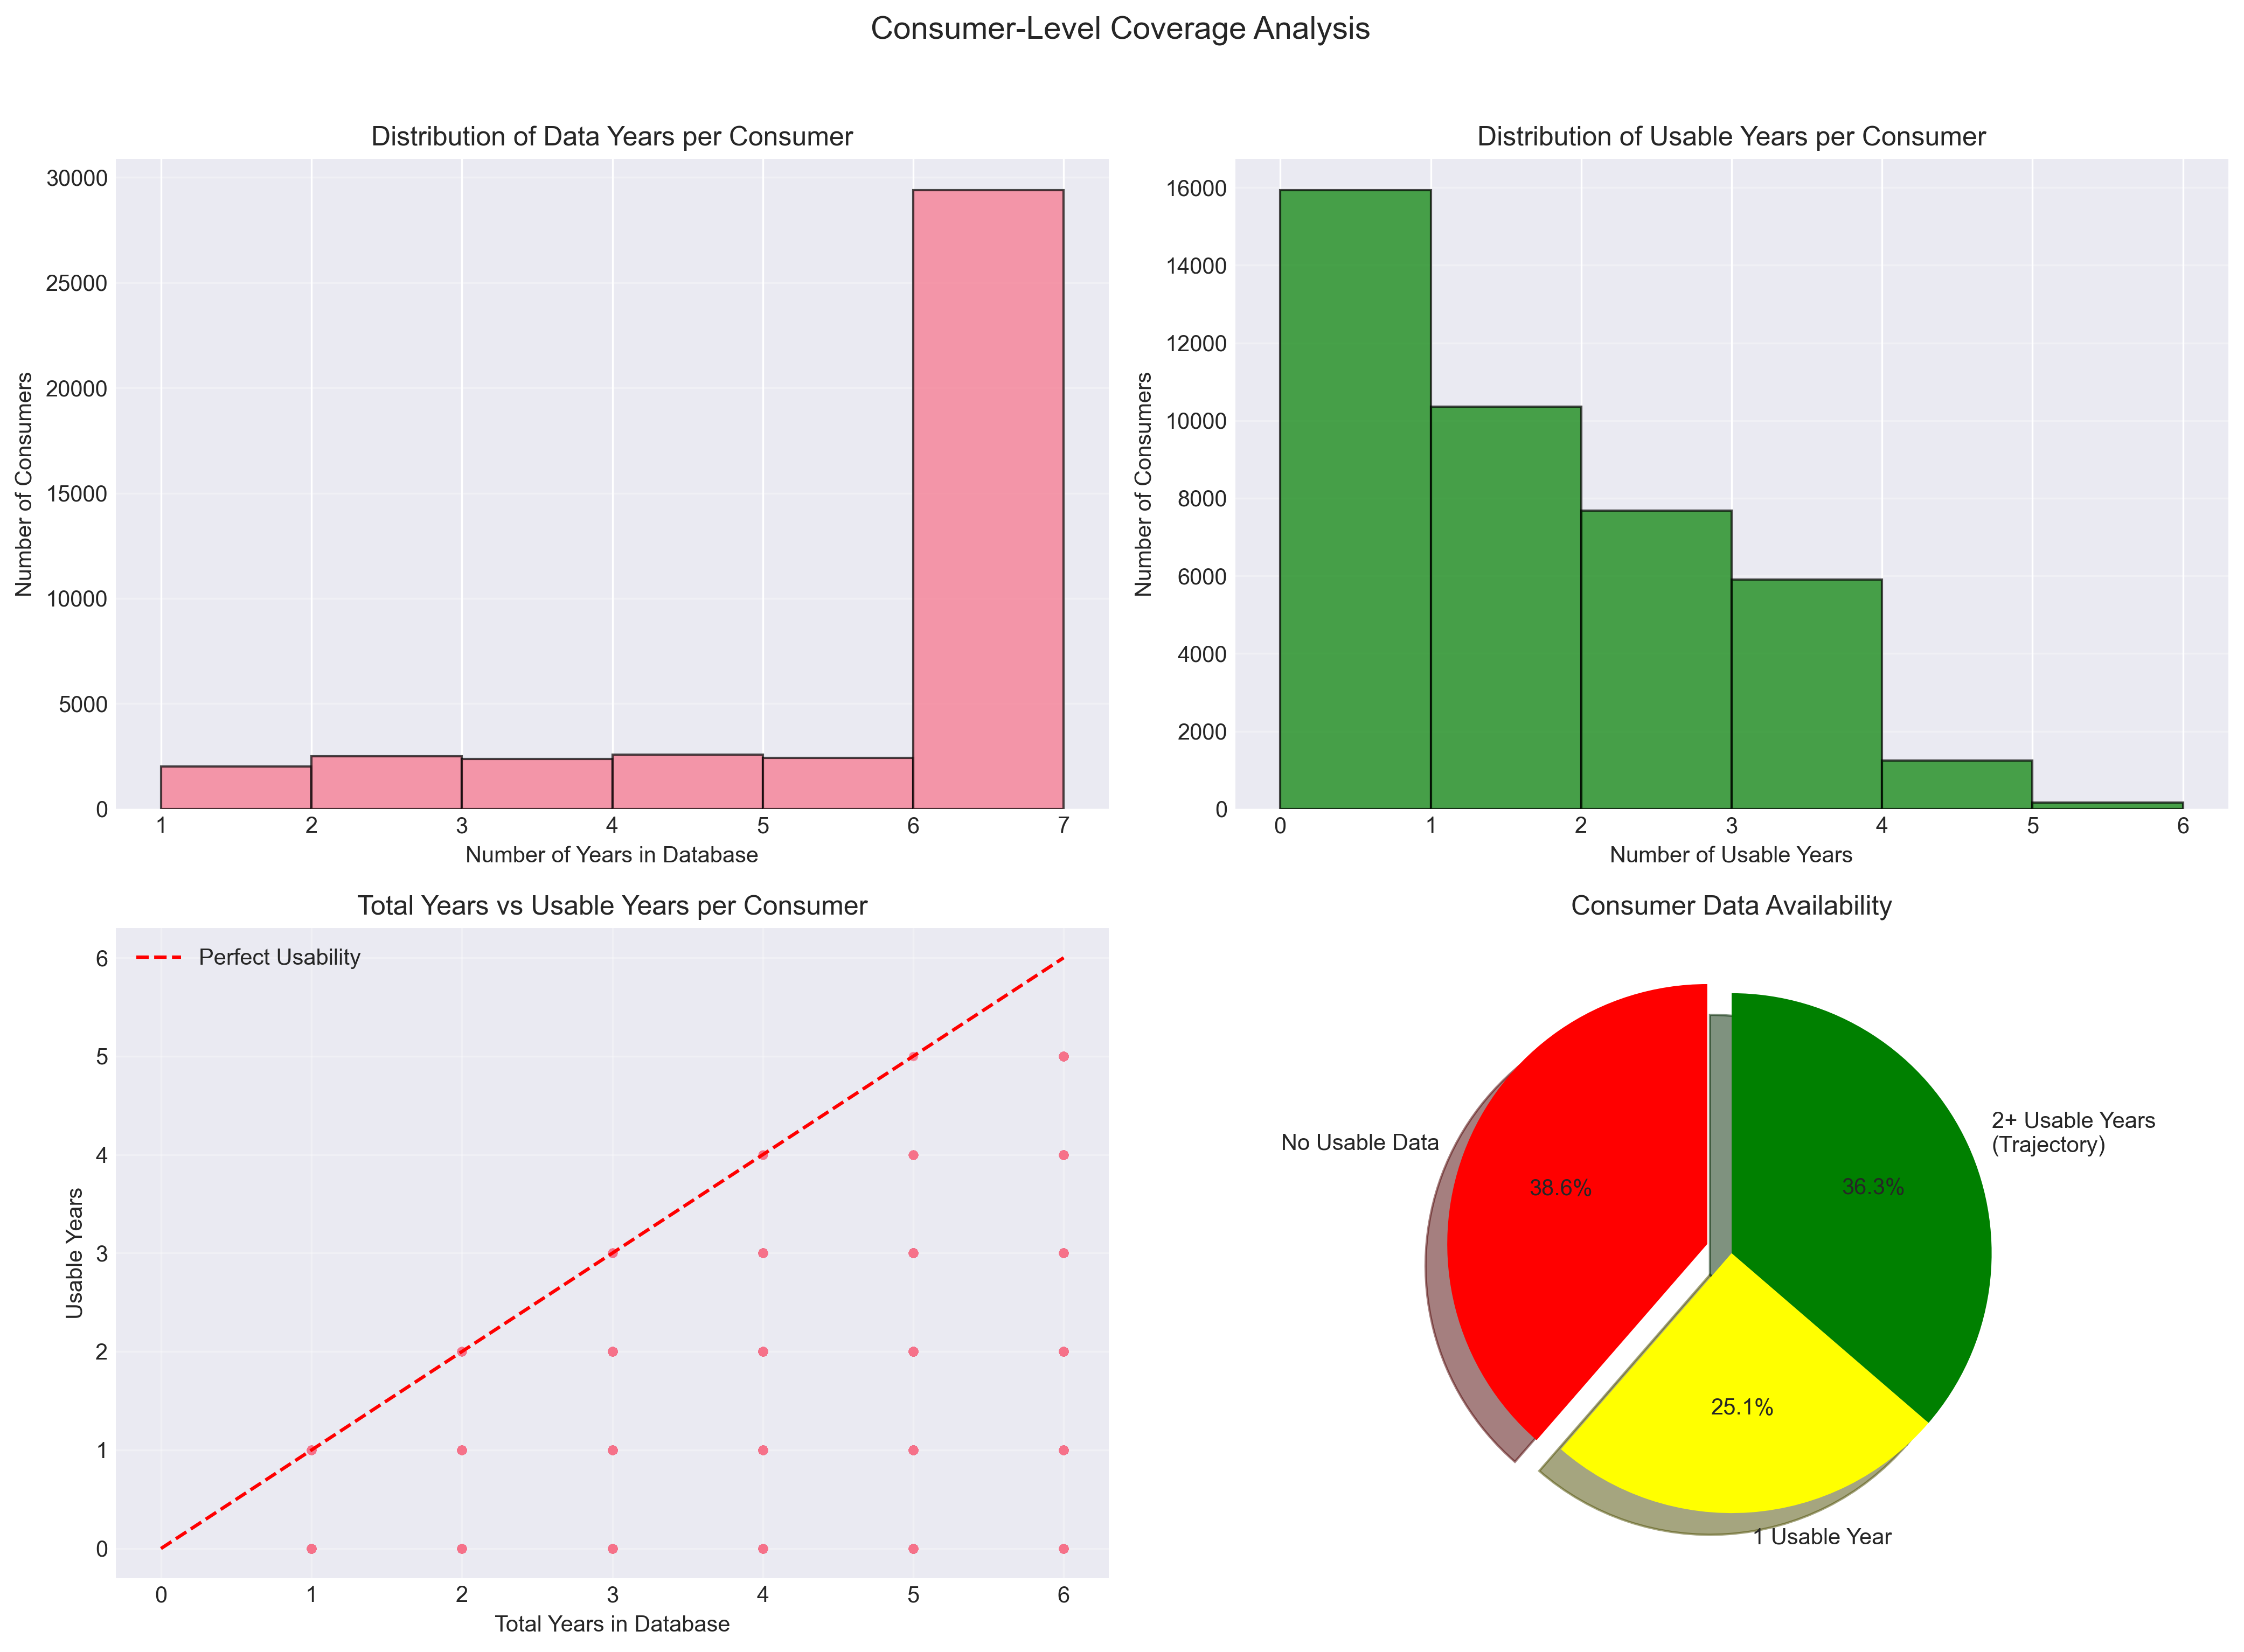
\includegraphics[width=\textwidth]{figures/consumer_coverage.png}
    \caption{Customer-level data coverage analysis}
    \label{fig:customer_coverage}
\end{figure}

Figure~\ref{fig:customer_coverage} presents four panels analyzing customer data availability:
\begin{itemize}
    \item \textbf{Top-left panel}: Distribution of total years each customer appears in the database, showing most customers have either 1-2 years or the full span of data
    \item \textbf{Top-right panel}: Distribution of usable years after applying quality criteria, revealing significant data loss for many customers
    \item \textbf{Bottom-left panel}: Scatter plot comparing total versus usable years, with the red diagonal line representing perfect data usability; points below the line indicate data quality issues
    \item \textbf{Bottom-right panel}: Pie chart showing the critical breakdown---only \CustomerPctTwoPlusYear\% of customers have sufficient data for trajectory modeling
\end{itemize}

\subsection{Data Exclusion Analysis}

Customer-year records are evaluated for several quality issues that would compromise model calibration:

\begin{table}[h]
\centering
\caption{Exclusion Reasons and Impact}
\begin{tabular}{lrr}
\toprule
\textbf{Exclusion Reason} & \textbf{Count} & \textbf{Percentage} \\
\midrule
Mid-Year QSI Change & \ExclusionMidYearQSICount & \ExclusionMidYearQSIPct\% \\
Late Entry (>30 days) & \ExclusionLateEntryCount & \ExclusionLateEntryPct\% \\
Early Exit (>30 days) & \ExclusionEarlyExitCount & \ExclusionEarlyExitPct\% \\
No Costs Recorded & \ExclusionNoCostsCount & \ExclusionNoCostsPct\% \\
Insufficient Service Days & \ExclusionInsufficientServiceCount & \ExclusionInsufficientServicePct\% \\
No QSI Assessment & \ExclusionNoQSICount & \ExclusionNoQSIPct\% \\
\bottomrule
\end{tabular}
\end{table}

\begin{figure}[h]
    \centering
    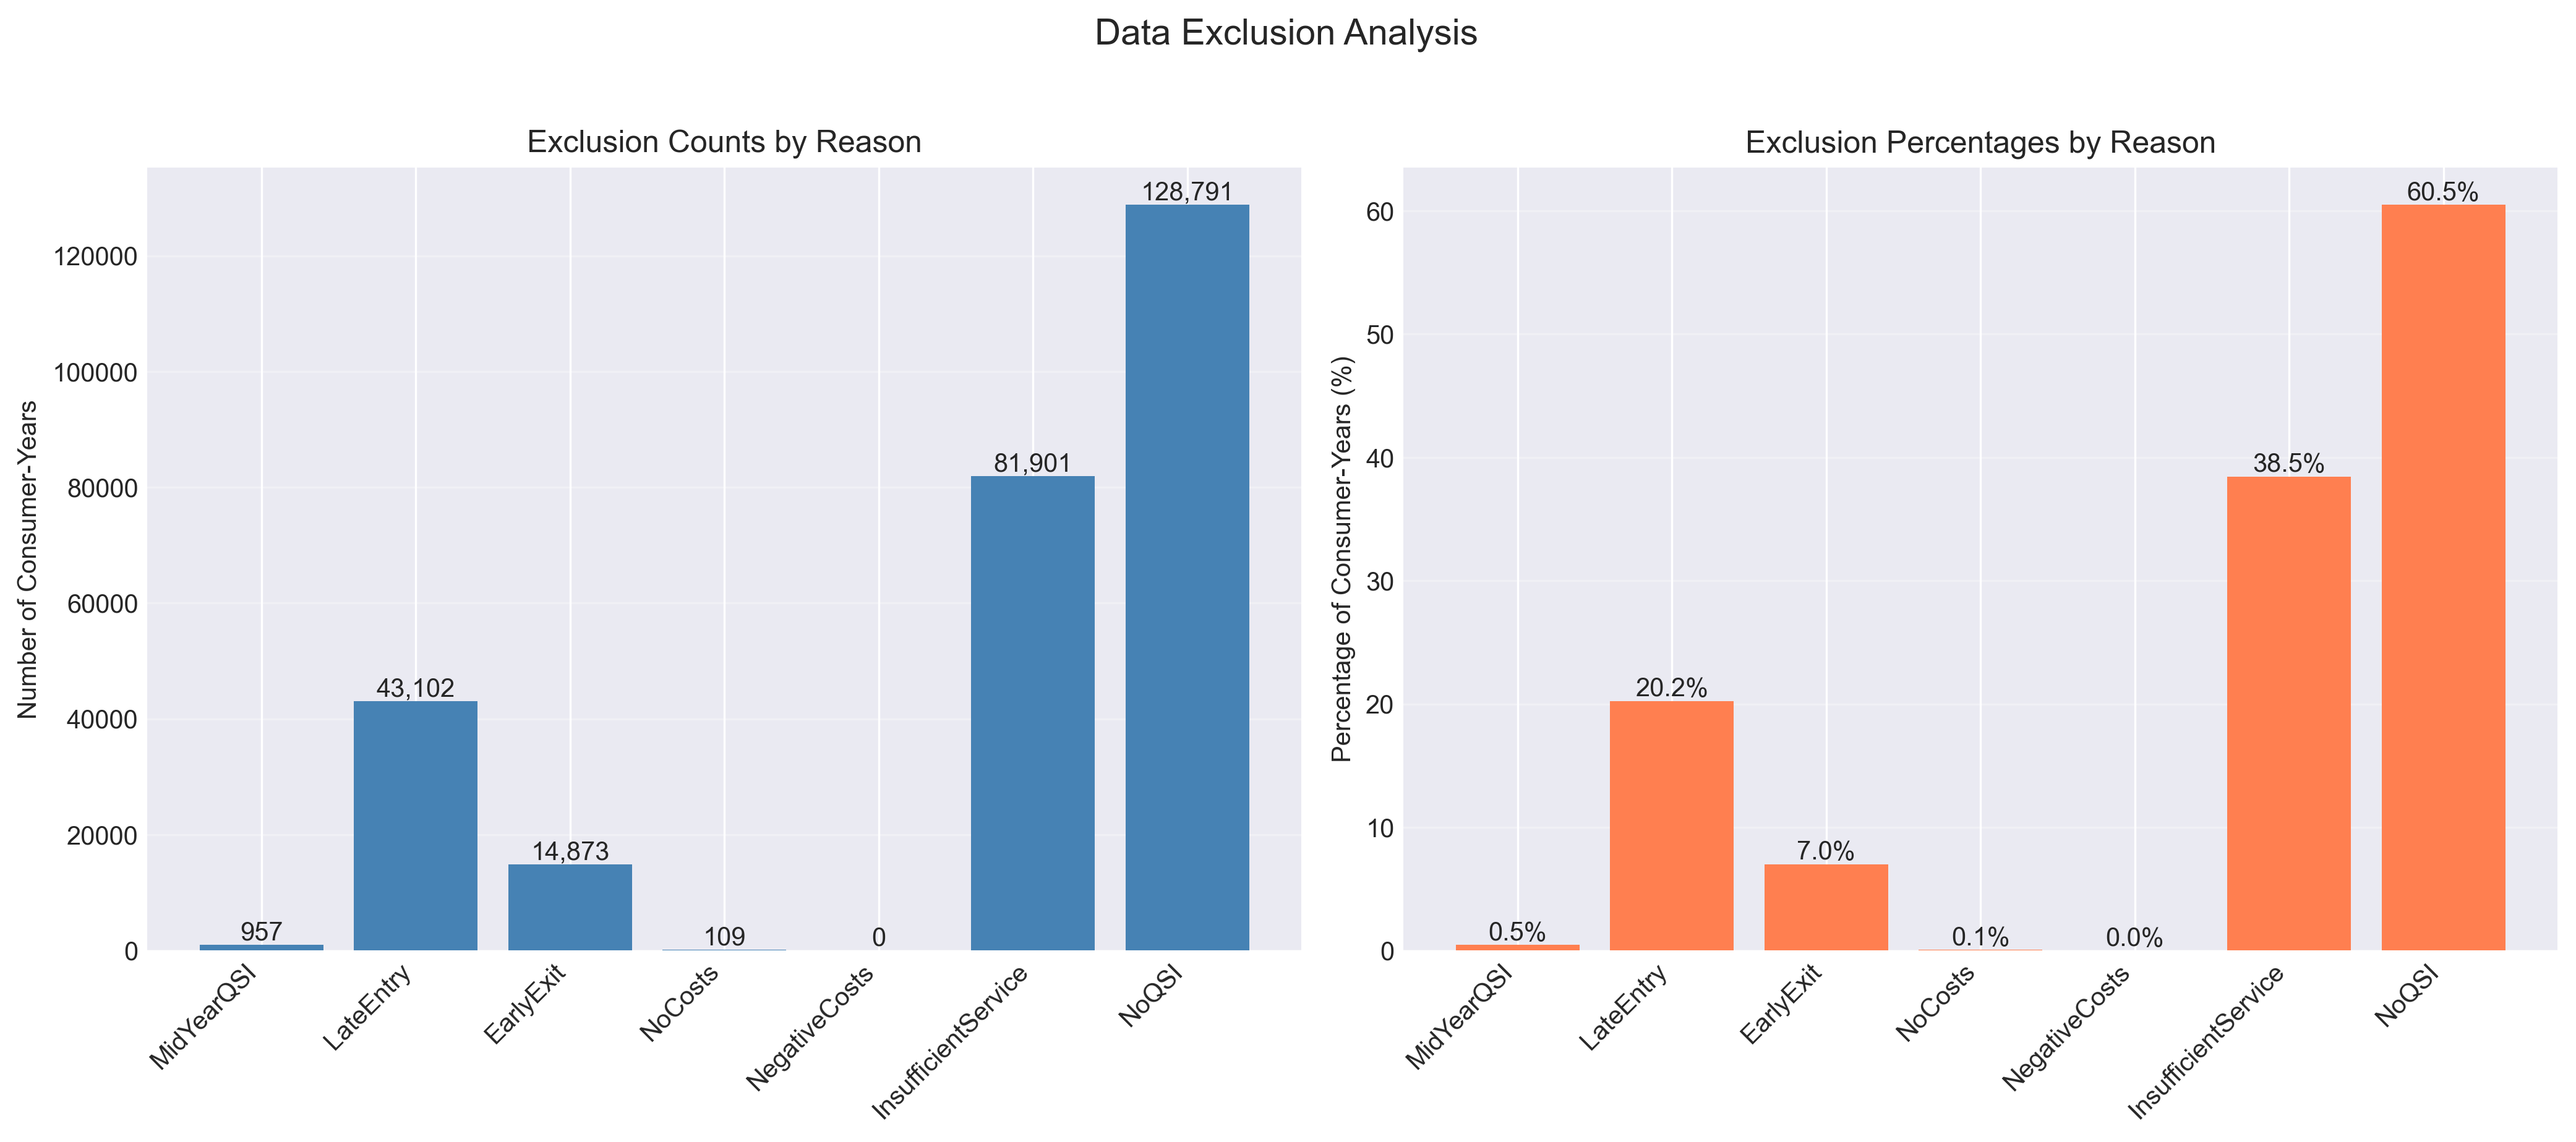
\includegraphics[width=\textwidth]{figures/exclusion_reasons.png}
    \caption{Distribution of exclusion reasons}
    \label{fig:exclusion_reasons}
\end{figure}

Figure~\ref{fig:exclusion_reasons} visualizes the exclusion analysis:
\begin{itemize}
    \item \textbf{Left panel}: Absolute counts of customer-years excluded for each reason, showing the scale of data loss
    \item \textbf{Right panel}: Percentage breakdown highlighting that mid-year QSI changes and incomplete fiscal years are the primary exclusion drivers
\end{itemize}

\subsection{Cost Distribution Analysis}

\begin{figure}[h]
    \centering
    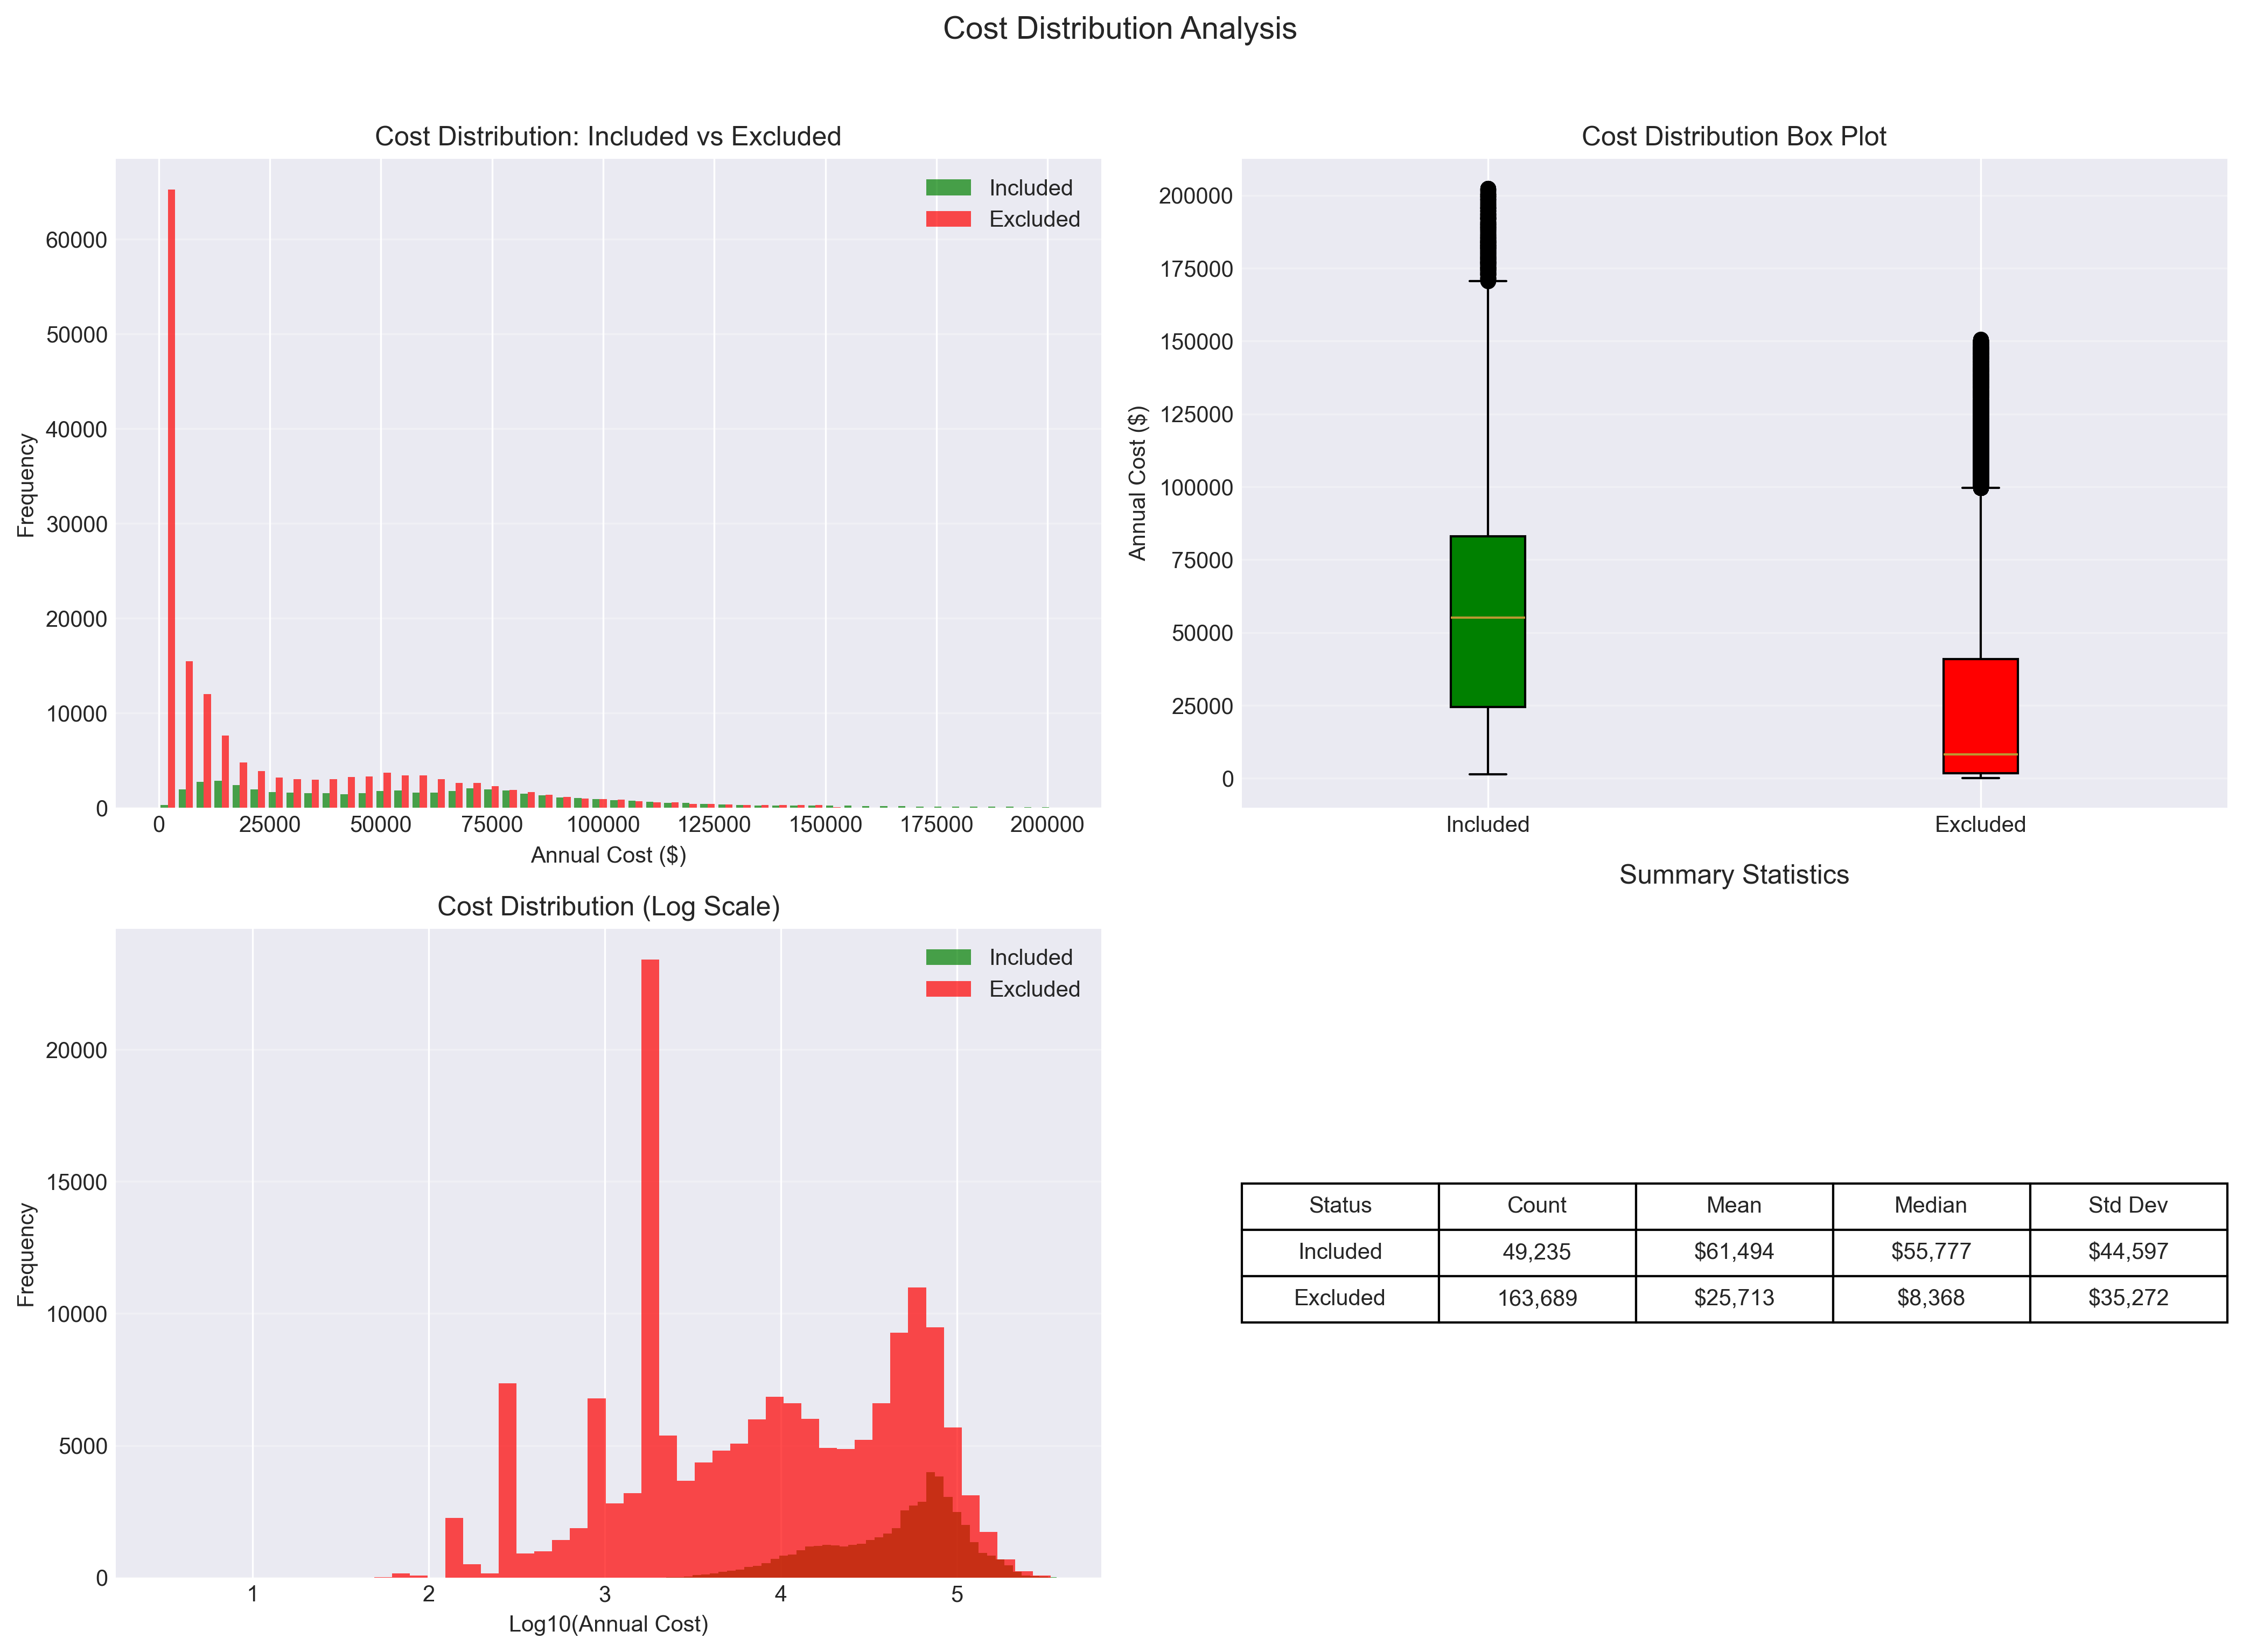
\includegraphics[width=\textwidth]{figures/cost_distributions.png}
    \caption{Comparison of cost distributions between included and excluded customer-years}
    \label{fig:cost_distributions}
\end{figure}

Figure~\ref{fig:cost_distributions} compares cost patterns between included and excluded data:
\begin{itemize}
    \item \textbf{Top-left}: Histogram overlay showing excluded records tend toward lower costs
    \item \textbf{Top-right}: Box plots revealing excluded records have wider variance and more outliers
    \item \textbf{Bottom-left}: Log-scale distribution highlighting the heavy tail in both populations
    \item \textbf{Bottom-right}: Summary statistics confirming systematically different cost profiles
\end{itemize}

\subsection{Temporal Trends}

\begin{figure}[h]
    \centering
    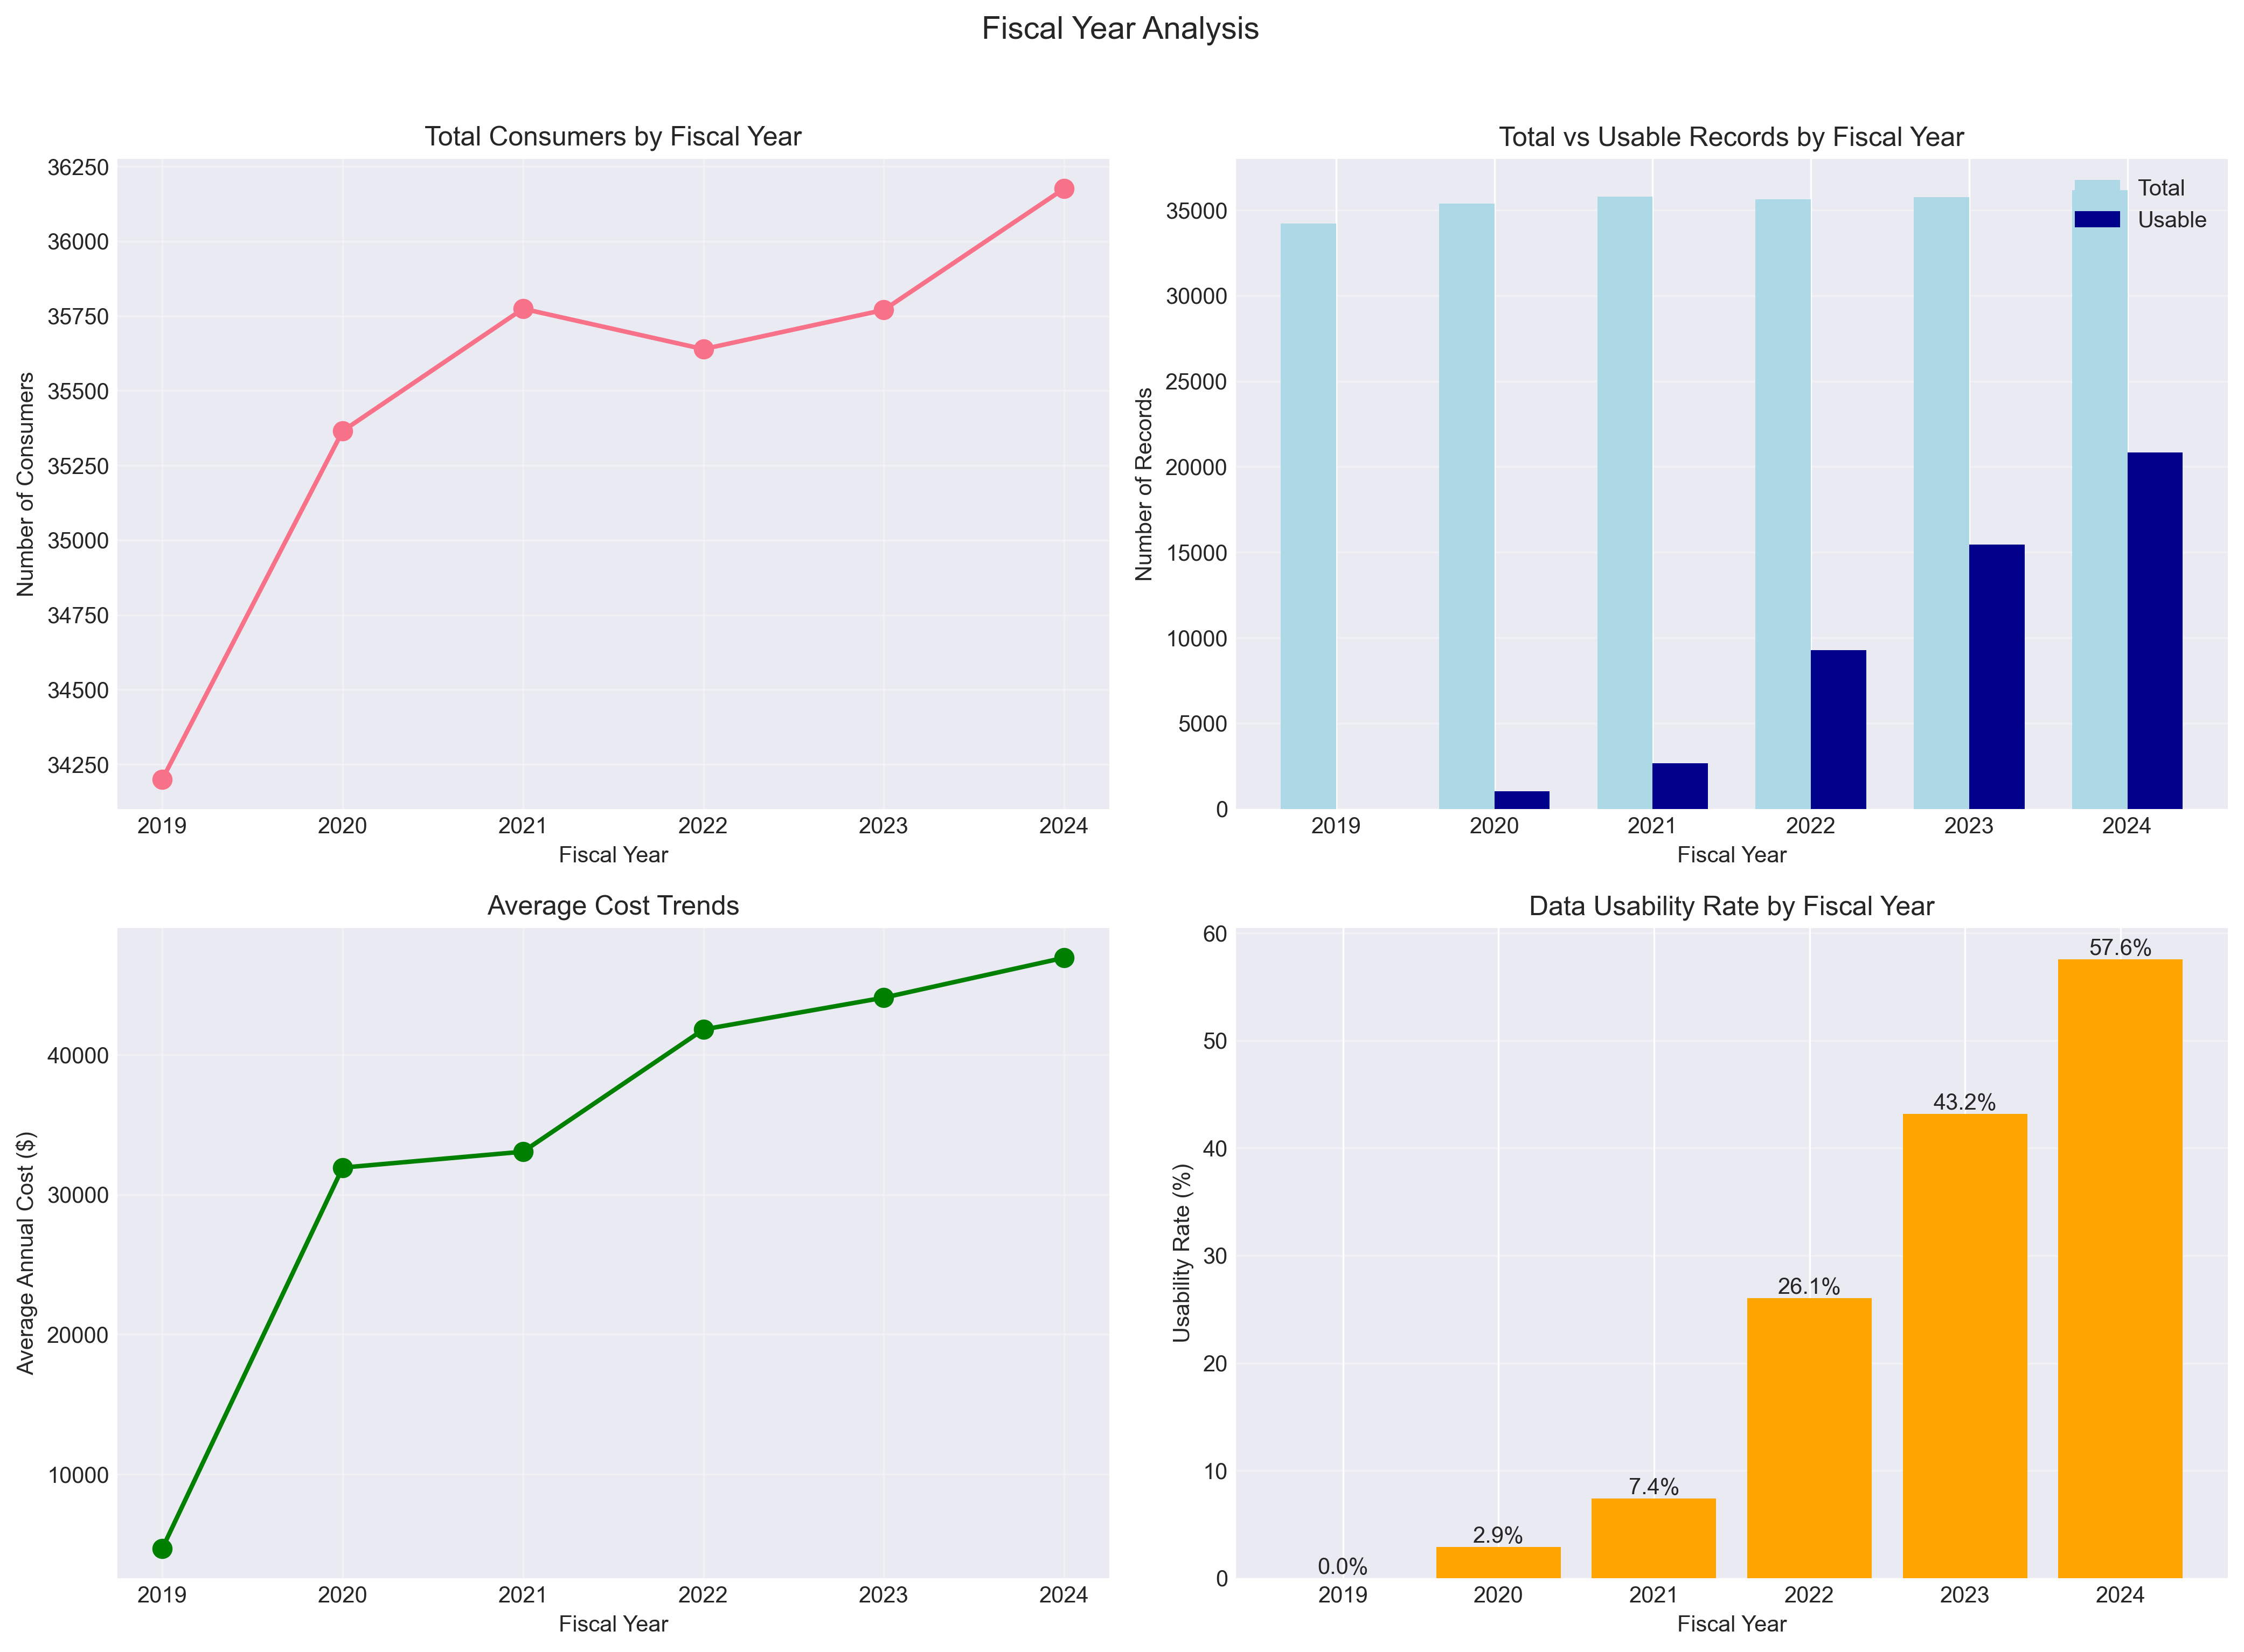
\includegraphics[width=\textwidth]{figures/fiscal_year_trends.png}
    \caption{Trends across fiscal years}
    \label{fig:fiscal_year_trends}
\end{figure}

Figure~\ref{fig:fiscal_year_trends} examines patterns over time:
\begin{itemize}
    \item \textbf{Top-left}: Customer counts by fiscal year show program growth
    \item \textbf{Top-right}: Comparison of total versus usable records reveals consistent data quality challenges
    \item \textbf{Bottom-left}: Average costs trending upward, reflecting inflation and service expansion
    \item \textbf{Bottom-right}: Data usability rates remain relatively stable across years
\end{itemize}

\subsection{Cost Outlier Analysis}

Using the Tukey method with a 3$\times$IQR threshold for extreme outliers:
\begin{itemize}
    \item Lower fence: \OutlierLowerFence
    \item Upper fence: \OutlierUpperFence
    \item Outliers below lower fence: \OutliersBelow
    \item Outliers above upper fence: \OutliersAbove
    \item Total outlier rate: \OutlierRate\%
\end{itemize}

\begin{figure}[h]
    \centering
    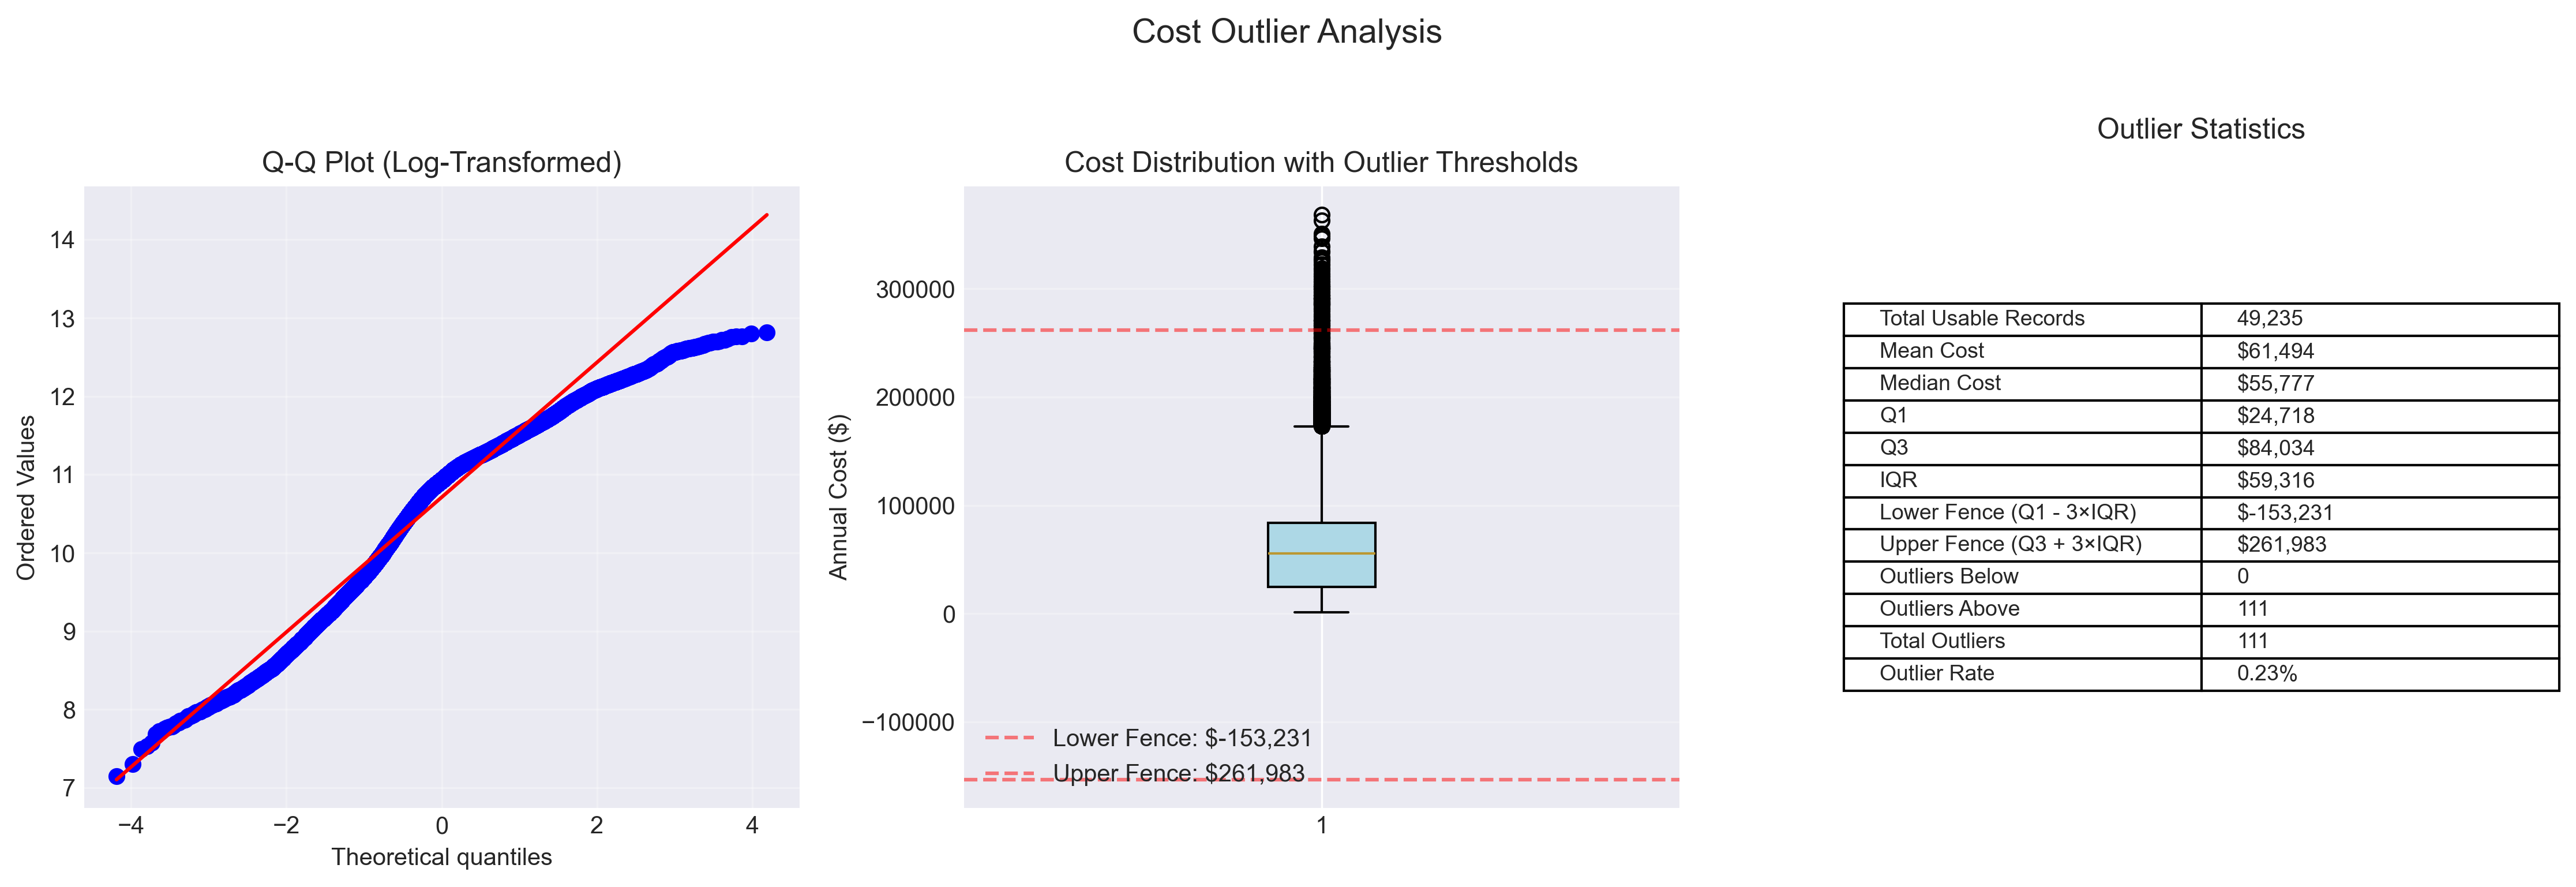
\includegraphics[width=\textwidth]{figures/cost_outliers.png}
    \caption{Cost outlier analysis}
    \label{fig:cost_outliers}
\end{figure}

Figure~\ref{fig:cost_outliers} provides outlier diagnostics:
\begin{itemize}
    \item \textbf{Left panel}: Q-Q plot of log-transformed costs shows approximate normality with heavy tails
    \item \textbf{Center panel}: Box plot with outlier thresholds (red dashed lines) identifies extreme values
    \item \textbf{Right panel}: Statistical summary quantifying outlier prevalence
\end{itemize}

\subsection{Exclusion Overlap Analysis}

\begin{figure}[h]
    \centering
    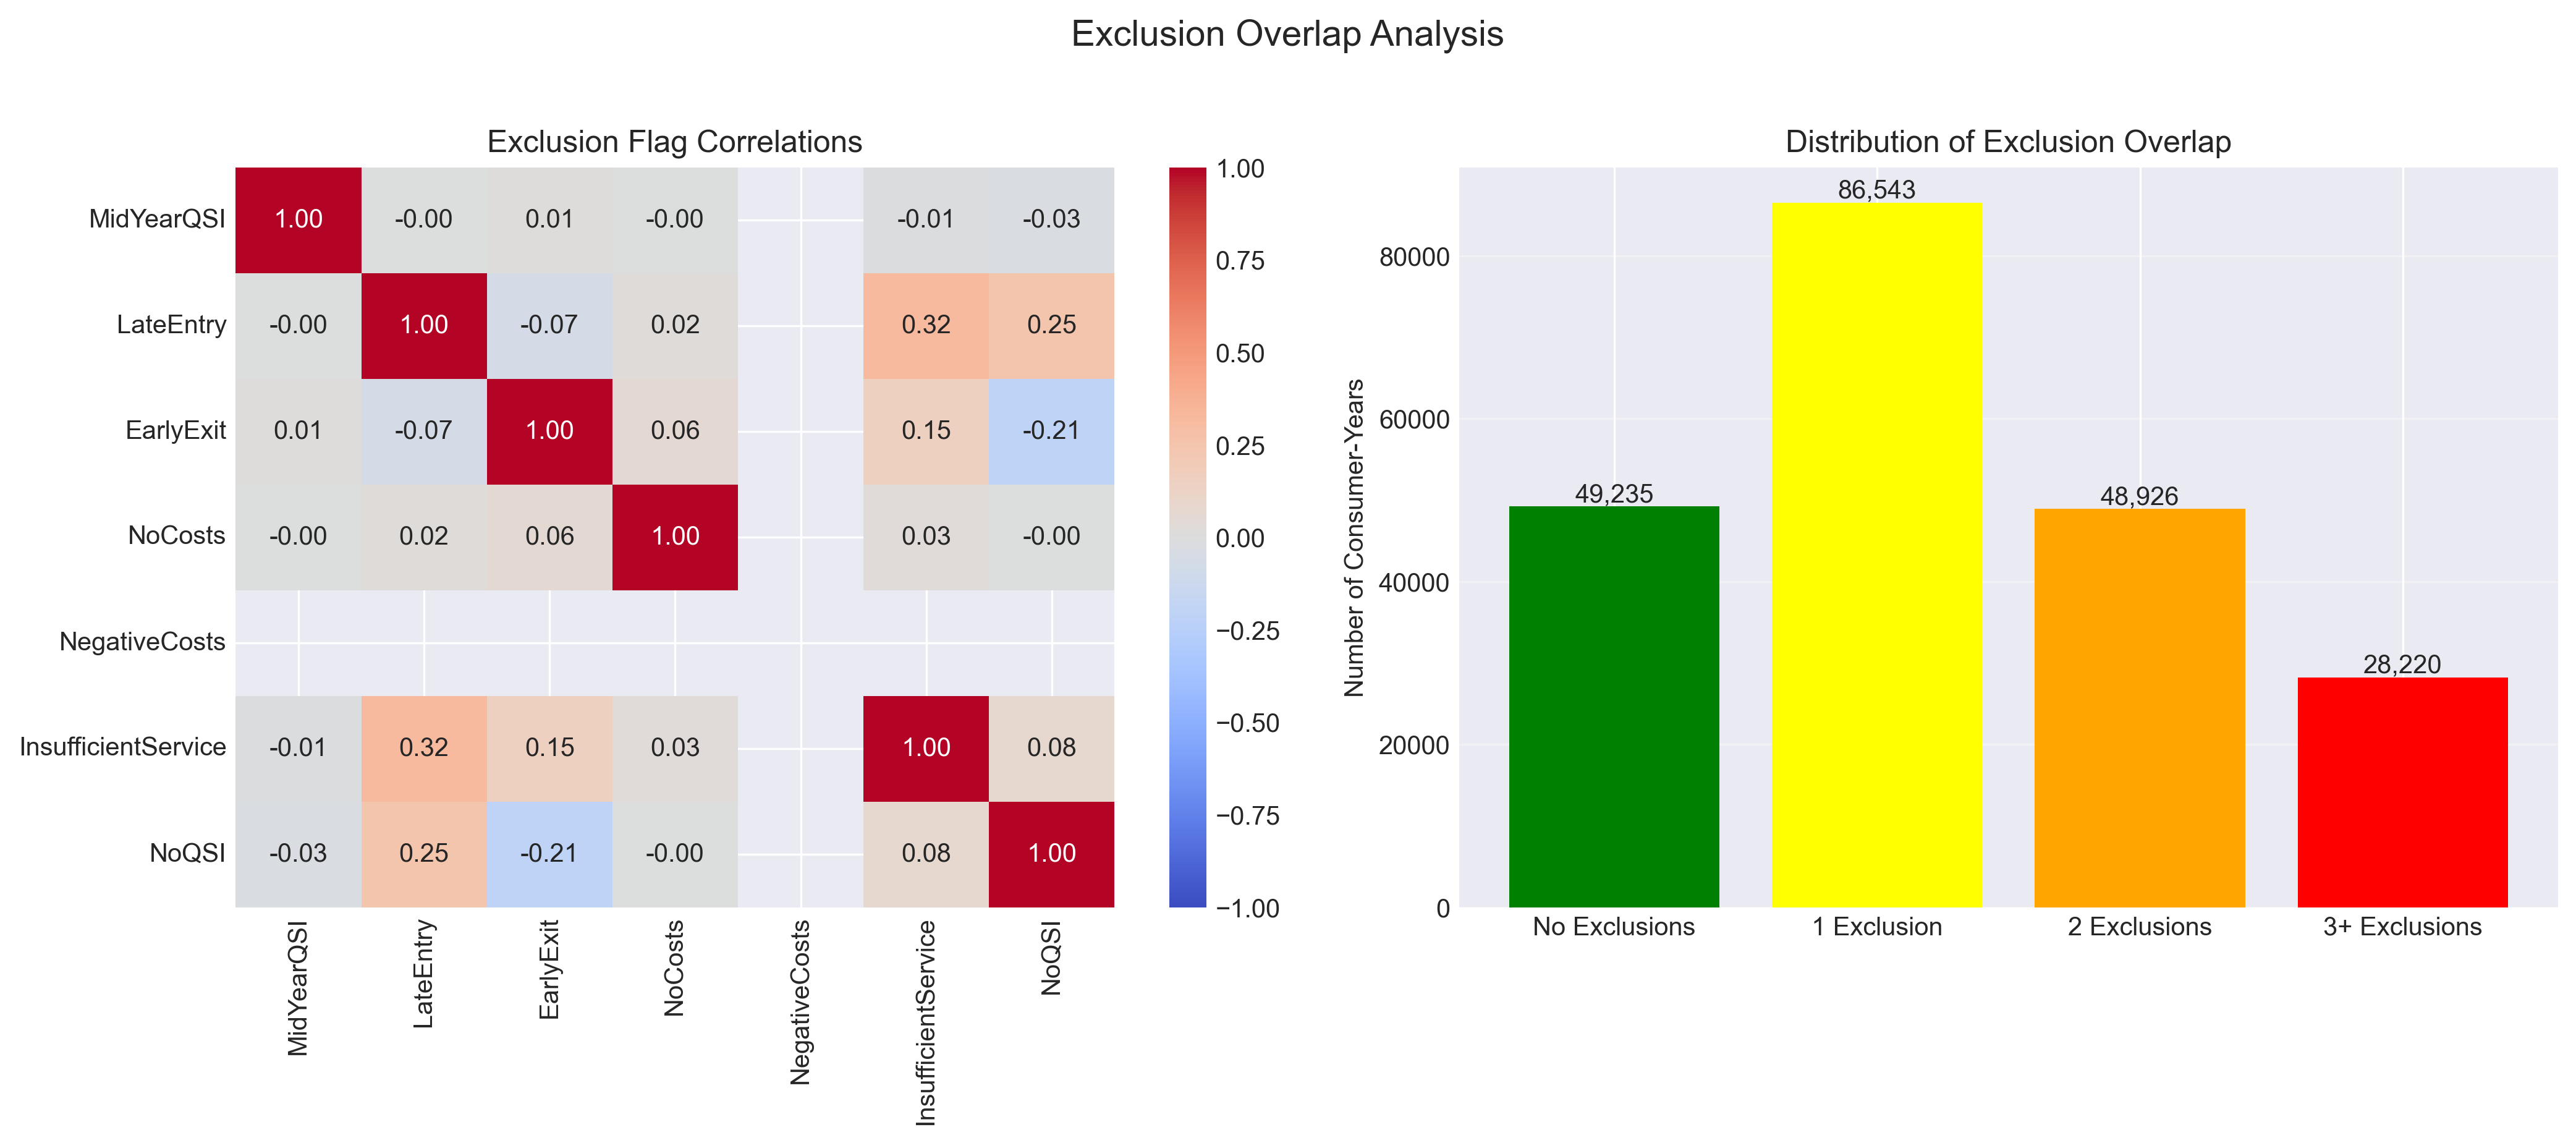
\includegraphics[width=\textwidth]{figures/exclusion_overlap.png}
    \caption{Analysis of exclusion flag correlations and overlap}
    \label{fig:exclusion_overlap}
\end{figure}

Figure~\ref{fig:exclusion_overlap} examines relationships between exclusion criteria:
\begin{itemize}
    \item \textbf{Left panel}: Correlation heatmap reveals which exclusion reasons tend to co-occur (red indicates positive correlation)
    \item \textbf{Right panel}: Bar chart showing most excluded records have multiple issues, justifying the conservative approach
\end{itemize}

\subsection{Trajectory Analysis Feasibility}

For the proposed individual trajectory modeling:
\begin{itemize}
    \item \textbf{\CustomersWithTrajectory{} customers (\PctWithTrajectory\%)} have sufficient data for individual trajectory calculation
    \item \textbf{\CustomersWithGaps{} customers (\PctWithGaps\%)} have gaps in their yearly data
    \item Customers without multi-year data will require group-based trajectory imputation
\end{itemize}

\subsection{Recommendations}

Based on this analysis:

\begin{enumerate}
    \item \textbf{Data Sufficiency}: With \CustomerPctOneYear\% of customers having usable data and \CustomerPctTwoPlusYear\% having multi-year data, the dataset supports model calibration but requires careful handling of limited trajectory coverage.
    
    \item \textbf{Trajectory Modeling}: The proposed trajectory approach is feasible for approximately \PctWithTrajectory\% of customers. The remaining customers will require cluster-based imputation.
    
    \item \textbf{Exclusion Strategy}: The conservative approach excluding customer-years with mid-year QSI changes affects \ExclusionMidYearQSIPct\% of records but ensures clean QSI-to-cost mapping.
    
    \item \textbf{Model Robustness}: Models should be tested for sensitivity to the exclusion criteria and validated on both included and excluded populations where feasible.
\end{enumerate}
